\fontsize{13px}{13px}\selectfont\justifying
\section{Đặc tả}
đồ án giải quyết vấn đề tạo trang thương mại điện tử cho chính nhà cung cấp. Và liên kết sản phẩm để phân phối thông tin giữa các nhà bán hàng dùng chung hệ thống đồ án này. Khi một người bắt đầu đăng ký hộ kinh doanh hoặc doanh nghiệp để sản xuất và cung cấp sản phẩm ra thị trường. Thì để thiết lập một trang bán hàng riêng, người đó chỉ cần thuê dịch vụ tên miền ở một nhà cung cấp bất kì. Đăng ký tài khoản và chờ duyệt trở thành nhà bán hàng. Sau khi được duyệt, nhà sản xuất có thể đăng tải thông tin và cung cấp quyền cài đặt tên miền đề liên kết trình bày dữ liệu của nhà sản xuất lên tại tên miền đó. Chi phí khởi tạo và duy trì là miễn phí. Khi doanh nghiệp thực sự cần và đã khai thác được nguồn lợi từ việc quảng bá trang thương mại điện tử. Hệ thống phần mềm có cơ chế mở rộng tài nguyên sử dụng cho nhà sản xuất.

Tiếp đến khi một nhà sản xuất, hoặc một cửa hàng có tài khoản nhà bán hàng trên hệ thống. Họ có nhu cầu đăng tải sản phẩm của tối tác trên trang thông tin của mình để tiếp thị sản phẩm cho khách hàng truy cập trang được đa dạng hơn. Người đó cần tạo một lời mời ký gửi thông tin đến nhà sản xuất sản phẩm đó. Sau khi được duyệt, các sản phẩm của nhà sản xuất đã hiện thì và có thể đặt hàng ở trên trang của đối tác.

Sau khi nhận được đơn đặt hàng, cùng với sản phẩm nằm ngoài doanh mục mà cửa hàng hoặc nhà sản xuất đó cung cấp. Người xử lý đơn có thể chuyển tiếp đơn đó cho đối tác xử lý như một hình thức \gls{dropshipping}.

Khách hàng truy cập vào trang sẽ thấy thông tin như một trang thương mại điện tử thông thường, các trang thương mại điện tử này dùng chung dữ liệu nên một tài khoản có thể đăng nhập trên nhiều trang. Tạo ra sự đăng nhập liền mạch cải thiện trải nghiệm người dùng.

%\begin{figure}[h!]\fontsize{13px}{13px}\selectfont
%	\begin{center}	
%		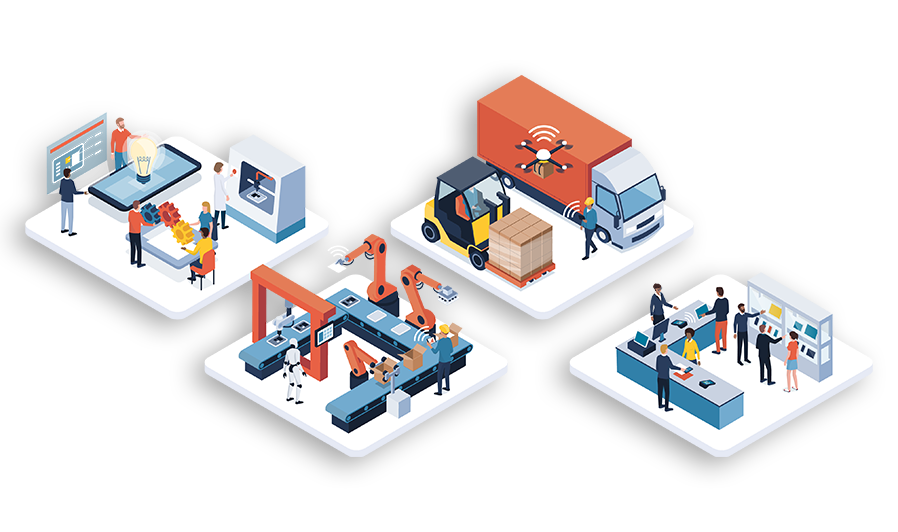
\includegraphics[width=0.6\textwidth]{manufacture}
%		\caption{Minh họa mô hình sản xuất và bán hàng}
%	\end{center}
%\end{figure}
\subsection{Yêu cầu tính năng}
Các tính năng yêu cầu có thể được liệt kê ra như sau:
\begin{itemize}
	\item Đăng nhập, đăng xuất, đăng ký, quên mật khẩu.
	\item Quản lý các thông tin liên quan đến sản phẩm và bài viết.
	\item Yêu cầu đối tác liên kết thông tin với nhau. Chấp nhận liên kết hoặc xóa.
	\item Khách hàng có thể xem và đặt sản phẩm ở các trang khác nhau.
	\item Có trang quản trị chung cho các nhà bán hàng xem đơn đặt hàng trên trang thương mại điện tử của họ.
	\item Nhà bán hàng có thể gửi thư điện tử cho những người có liên kết bạn bè.
	\item Hệ thống có thể gửi thư điện tử thông báo đơn hàng.
	\item Yêu cầu mở tài khoản cho nhà bán hàng nhanh và tự động. Hạn chế sự can thiệp về mặt kỹ thuật của nhà phát triển.
	\item Yêu cầu đo lường được hoạt động của người dùng hệ thống.
	\item Sản phẩm có thể có nhiều thuộc tính tùy chọn khi mua hàng.
	\item Có thể cài đặt hiển thị số lượng tồn kho của sản phẩm trên trang.
	\item Có thể tự tùy chỉnh hầu hết các nội dung trên trang ngoại trừ các chỉnh sửa về mặt đồ họa, giao diện, bố cục của trang.
\end{itemize}
\subsection{Yêu cầu giao diện}
\begin{itemize}
	\item Giao diện cần được thiết kế hiện đại và dễ sử dụng.
	\item Tương thích ít nhất 80\% các loại màn hình.
	\item Mức độ hoàn thiện tương thích màn hình ít nhất 70\%.
	\item Thao tác nút bấm to rõ và hạn chế bị giật khi tải lại các thành phần của trang.
	\item Tăng các thành phần phản ứng với hành động của người dùng để tạo cảm giác hệ thống đang xử lý liền mạch không bị chậm chạp.
\end{itemize}
\subsection{Yêu cầu hiệu suất}
\begin{itemize}
	\item Tất cả các tương tác của người dùng không được phản hồi chậm quá 3 giây.
	\item Tất cả phản hồi có thể đợi quá 5 giây cần được phản hồi lại tiến độ hoàn thành. Hoặc tình trạng truy vấn.
	\item Các thay đổi dữ liệu không được cập nhật chậm hơn 5 phút sau khi sửa đổi.
\end{itemize}

\subsection{Yêu cầu thiết kế}
\begin{itemize}
	\item Hệ thống sử dụng các công nghệ còn được duy trì và phát triển.
	\item Hệ thống có thể chia nhỏ ra thành các đội nhóm khi trở nên quá lớn.
	\item Hệ thống có thể nâng cấp theo chiều ngang với các lựa chọn có chi phí hợp lý.
	\item Hệ thống không bị phụ thuộc và có phương pháp phát triển dự phòng.
\end{itemize}

\subsection{Yêu cầu phi tính năng}
\begin{itemize}
	\item Mã hóa thông tin mật khẩu.
	\item Sao lưu dự phòng dữ liệu hằng tháng.
	\item Sao lưu dự phòng tiến trình thực thi ổn định.
\end{itemize}

\subsection{Vai trò}
\subsubsection{Người bán hàng}
Người bán hàng là người có quyền công bố dữ liệu của họ cho mọi người truy cập thông qua một tên miền cụ thể.

Người bán hàng có thể mời người bán hàng khác, gộp dữ liệu sản phẩm của họ vào bày bán ở trang của mình. Hoặc cũng có thể tham giam đóng góp sản phẩm của mình vào các sàn bán hàng của những người bán hàng khác.

\subsubsection{Người mua hàng}
Người mua hàng là người thực hiện các hoạt động xem thông tin, tạo giỏ hàng, thêm sản phẩm vào giỏ hàng và đặt mua. Người mua hàng không cần thiết phải đăng nhập vào hệ thống. Chỉ cần để lại thông tin địa chỉ để giao hàng là được. Vì hiện tại, hai hình thức thanh toán chuyển khoản và thanh toán \acrshort{cod} rất an toàn cho người bán. Nếu có rủi ro thì chi phí vận chuyển là không quá lớn.

Người mua hàng nếu chủ động lưu trữ thông tin đơn hàng hoặc các hoạt động để cá nhân hóa dữ liệu thì có thể đăng nhập trước khi thực hiện các thành động liên quan.

\subsection{Hoạt động}
Giống như các hệ thống khác, hoạt động được chia ra thành tạo, xem, sửa, xóa. Các hoạt động này được xác định là xảy ra ở tên miền nào, dữ liệu đối tượng gì, do ai có vai trò gì thực hiện.

Với cách xác định hoạt động như trên, có gần với khái niệm \emph{phương thức} của đối tượng trong quan niệm thiết kế hướng đối tượng.

\subsection{Phân quyền}

Phân quyền không chỉ giúp cho hệ thống trở nên bảo mật hơn. Mà còn giúp cho đội ngũ phát triển làm việc chặt chẽ hơn với dữ liệu. Một dạng dữ liệu được phân quyền với yêu cầu đặc tả của khách hàng không thể truyền đạt hết cho tất cả những thành viên trong nhóm được. Điều đó gây ra các lỗ hổng đằng sau \gls{controller} trong mô hình \acrshort{mvc}. Hệ thống sử dụng các nút xử lý mang theo thông tin chung đại diện cho người truy cập. Trong đó có thể phân tách định nghĩa được hoạt động và phân quyền được chặt chẽ hơn. Dưới đây là một số định nghĩa về phân quyền cần lưu ý:

\subsubsection{Quyền đại diện}\label{what-is-owner}
Khi thực hiện truy vấn dữ liệu, cần xác định nguồn gốc của truy vấn đến từ \gls{request} \cite{http} nào. Quyền đại diện cho truy vấn được cấp cho tài khoản nhà bán hàng có tên miền khớp với tên miền chứa trong \gls{request} đó. Tức là có thể lấy được ID của tài khoản đại diện cho \gls{request} hiện tại. 

Chỉ có tài khoản người bán hàng mới có thể đại diện cho một truy vấn. Khi người bán hàng truy vấn từ một trang không phải thuộc sở hữu của họ. Thì hệ thống thay vì căn cứ vào tên miền ở trong \gls{request} hiện tại như cách cũ, nó sẽ trả về luôn \gls{id} của người bán hàng hiện tại. Tức là ghi đè quyền đại diện nếu người thực hiện truy vấn là một nhà bán hàng.

Quyền đại diện thường được sử dụng để xem dữ liệu như một nhà bán hàng tại một tên miền cụ thể. Nghĩa là khi người dùng truy vấn dữ liệu sản phẩm tại một domain nào đó. Thì hệ thống sẽ hỏi cơ sở hữu liệu ai đại diện cho truy vấn này để trả về dữ liệu tương ứng cho truy vấn đó.

Điều này cho phép cùng một hệ thống máy chủ giao diện khi cài đặt với các tên miền khác nhau sẽ trả về các kết quả khác nhau.

Phân quyền này dựa trên chứng thực \gls{headers} của \gls{request}. Tức là nếu ở ứng dụng \gls{mobile} hoặc một nền tảng khác không chứng thực được \gls{headers}. Người dùng không thể giả mạo \gls{headers} để truy vấn thông tin của nhà bán hàng.

Nội dung và phương pháp chứng thực \gls{headers} \gls{request} nằm ngoài phạm vi đề cập của đồ án.

\subsubsection{Quyền hành động}

\textbf{Quyền sở hữu.} Đối với quyền sở hữu. Ai tạo ra dữ liệu thì người đó mới có quyền xóa dữ liệu đó. Cho nên tất cả các bảng đều phải có ghi thông tin người tạo. Bởi vì trong quá trình phát triển đồ án theo yêu cầu thực tế, mối liên hệ giữa các bảng có thể thay đổi nhưng quyền sở hữu giữa dữ liệu đó và người sở hữu không thay đổi. Nếu tạo ra dữ liệu mà không đăng nhập, không xác định được người sở hữu, thì dữ liệu sẽ thuộc về người đại diện cho truy cập (Xem chi tiết người đại diện của truy cập mục \ref{what-is-owner}).

\textbf{Chuyển quyền sở hữu.} Khi tạo đơn đặt hàng, tạo nội dung, dữ liệu sản phẩm cho người khác. Phải quyển quyền sở hữu sau đó. Sẽ có nghiệp vụ chạy ngầm để xét duyệt và ghi đè quyền sở hữu cho người thừa kế. Ghi thông tin người tạo vào dữ liệu vào một trường khác nếu cần. Nhưng bản chất dữ liệu đó đã chuyển quyền sở hữu rồi.

Nghĩa là, coi như người thừa kế (\emph{người được chuyển}) tạo ra dữ liệu đó. sau khi chuyển người sở hữu cũ không có quyền xóa nữa.

\textbf{Quyền xem.}\label{read:permission} đa dạng hơn tùy trường hợp sử dụng.

Quyền xem được thiết đặt theo thứ tự: mặc định, bảng dữ liệu, trường dữ liệu. Nếu định nghĩa quyền xem cho một bảng dữ liệu cụ thể, thì hệ thống sẽ thực hiện định nghĩa đó thay cho quyền mặc định. Tương tự, nếu một trường có định nghĩa quyền xem cho riêng nó, thì khi truy vấn bảng dữ liệu, định nghĩa quyền chỉ áp dụng cho của bảng. Sau đó nếu truy cập hợp lệ vào trường đó thì mới trả về được dữ liệu của trường.

Ví dụ cho trường hợp phân quyền cho trường dữ liệu là khi truy vấn đến bảng người dùng, người xem có thể xem tên, hình ảnh đại diện nhưng không thể xem số điện thoại và mật khẩu đã mã hóa.

Quyền xem chia ra làm hai loại là phân quyền trực tiếp và phân quyền gián tiếp.

\begin{itemize}
	\item Đối với phân quyền trực tiếp thì người tạo ra, người sở hữu dữ liệu toàn quyền xem với dữ liệu đó.
	\item Quyền xem gián tiếp là quyền cấp cho người xem dữ liệu mà không cần đăng nhập, hoặc đăng nhập nhưng không phải là nhà bán hàng.
	
	Người xem gián tiếp được định nghĩa là khi truy cập dữ liệu dưới một tên miền, thì thông qua tên miền để lấy được quyền truy cập đến các dữ liệu được chia sẻ của: người sở hữu tên miền và người chia sẻ dữ liệu cho tên miền. Hoặc có thể hiểu là người mua hàng đã thông qua tên miền để truy cập đến dữ liệu của nhà bán hàng. Hoặc ngược lại căn cứ theo tên miền tìm nhà bán hàng đại diện để phục vụ dữ liệu cho người dùng.
	
\end{itemize}

\textbf{Quyền tạo} Khi tạo dữ liệu, đối với một số bảng dữ liệu bắt buộc đăng nhập thì người dùng phải đăng nhập, hoặc là nhà bán hàng thì mới có thể tạo.

Cũng có trường hợp các loại dữ liệu không cần đăng nhập vẫn tạo được để tạo ra sự thuận tiện cho người mua hàng. Ví dụ thêm một sản phẩm vào giỏ hàng. Thực tế khi mua hàng tại các siêu thị, người mua hàng có thể yêu cầu mở thẻ thành viên hoặc là không.

Những dữ liệu không đăng nhập có thể xem bởi tất cả mọi người, nhưng những sản phẩm có thông tin người tạo cần được xem xét cho phép truy cập bởi một số người liên quan chẳng hạn như đơn hàng được tạo trên cửa hàng. Người chủ cửa hàng cần quyền xem đơn hàng đó.


\subsubsection{Dưới đây là các mô tả cụ thể hơn về phân quyền:}

\textbf{Người dùng} Người dùng có thể nhìn thấy thông tin cá nhân cơ bản của chính họ và của những người đã chấp nhận bạn bè.

\textbf{Lời mời kết bạn} Người tạo ra lời mời và người được mời có thể nhìn thấy lời mời đó.

\textbf{Hợp đồng} Hợp đồng tương tự như lời mời kết bạn chỉ người tạo ra và đối tác của người đó được xem dữ liệu.

\textbf{Các tương tác} Các tương tác được xem công khai cho tất cả mọi người nhưng chỉ người tạo ra mới được chỉnh sửa.

\textbf{Thông báo} Thông báo từ hệ thống đến người dùng chỉ được xem bởi chính người đó. Trong trường hợp gửi thông báo cho nhau thì người gửi và người nhận được xem thông báo đó.

\textbf{Nhóm} Nhóm được xem bởi người tham gia nhóm và người đã chấp nhận lời mời tham gia nhóm. Lời mời tham gia nhóm tương tự với lời mời kết bạn.

\textbf{Thống kê truy cập} Thống kê theo dõi truy cập của một cá nhân chỉ được truy cập quản lý bởi chính cá nhân đó.

\textbf{Các bảng công việc} Khi giữa các tài khoản người dùng và tài khoản nhà bán hàng có kí hợp đồng lao động, người dùng có thể tạo bảng để chấm công khi làm việc cho một nhà bán hàng nào đó. Nên nhà bán hàng và người chấm công có thể xem. Yêu cầu chốt công tạo ra bởi người chấm công nhưng không ai có thể xóa. Nhà bán hàng có thể cập nhật hoặc ghi chú vào bảng chốt công.

\textbf{Thông tin công khai} Các thông tin công khai là những thông tin được tạo ra bởi nhà bán hàng và công khai truy cập thông qua một tên miền cụ thể. Đối với các truy cập không có thông tin tên miền. Người dùng đó không có quyền truy cập vào dữ liệu công khai. Ngoại trừ trường hợp người dùng đó đăng nhập với tài khoản nhà bán hàng (xem thêm \textbf{quyền xem} tại mục \ref{read:permission}).
